\documentclass[hyperref, a4paper]{article}

\usepackage{geometry}
\usepackage{float}
\usepackage{titling}
\usepackage{titlesec}
% No longer needed, since we will use enumitem package
% \usepackage{paralist}
\usepackage{enumitem}
\usepackage{footnote}
% \usepackage{enumerate}
\usepackage{amsmath, amssymb, amsthm}
\usepackage{mathtools}
\usepackage{bbm}
\usepackage{cite}
\usepackage{graphicx}
\usepackage{subcaption}
\usepackage{physics}
\usepackage{tensor}
\usepackage{siunitx}
\usepackage{booktabs}
\usepackage[version=4]{mhchem}
\usepackage{tikz}
\usepackage{xcolor}
\usepackage{listings}
\usepackage{autobreak}
\usepackage[ruled, vlined, linesnumbered]{algorithm2e}
\usepackage{xr-hyper}
\usepackage[colorlinks,unicode]{hyperref} % , linkcolor=black, anchorcolor=black, citecolor=black, urlcolor=black, filecolor=black
\usepackage[most]{tcolorbox}
\usepackage{prettyref}

% Page style
\geometry{left=3.18cm,right=3.18cm,top=2.54cm,bottom=2.54cm}
\titlespacing{\paragraph}{0pt}{1pt}{10pt}[20pt]
\setlength{\droptitle}{-5em}
\preauthor{\vspace{-10pt}\begin{center}}
\postauthor{\par\end{center}}

% More compact lists 
\setlist[itemize]{itemindent=17pt, leftmargin=1pt}

% Math operators
\DeclareMathOperator{\timeorder}{\mathcal{T}}
\DeclareMathOperator{\diag}{diag}
\DeclareMathOperator{\legpoly}{P}
\DeclareMathOperator{\primevalue}{P}
\DeclareMathOperator{\sgn}{sgn}
\newcommand*{\ii}{\mathrm{i}}
\newcommand*{\ee}{\mathrm{e}}
\newcommand*{\const}{\mathrm{const}}
\newcommand*{\suchthat}{\quad \text{s.t.} \quad}
\newcommand*{\argmin}{\arg\min}
\newcommand*{\argmax}{\arg\max}
\newcommand*{\normalorder}[1]{: #1 :}
\newcommand*{\pair}[1]{\langle #1 \rangle}
\newcommand*{\fd}[1]{\mathcal{D} #1}
\DeclareMathOperator{\bigO}{\mathcal{O}}
\DeclareMathOperator{\object}{Ob}
\DeclareMathOperator{\morphism}{Hom}

% TikZ setting
\usetikzlibrary{arrows,shapes,positioning}
\usetikzlibrary{arrows.meta}
\usetikzlibrary{decorations.markings}
\tikzstyle arrowstyle=[scale=1]
\tikzstyle directed=[postaction={decorate,decoration={markings,
    mark=at position .5 with {\arrow[arrowstyle]{stealth}}}}]
\tikzstyle ray=[directed, thick]
\tikzstyle dot=[anchor=base,fill,circle,inner sep=1pt]

% Algorithm setting
% Julia-style code
\SetKwIF{If}{ElseIf}{Else}{if}{}{elseif}{else}{end}
\SetKwFor{For}{for}{}{end}
\SetKwFor{While}{while}{}{end}
\SetKwProg{Function}{function}{}{end}
\SetArgSty{textnormal}

% Support for tensor double arrows.
\renewcommand{\tensor}[1]{ \stackrel{\leftrightarrow}{\vb*{#1}}}

\newcommand*{\concept}[1]{{\textbf{#1}}}

% Omit the page number
% \newrefformat{fig}{Figure~\ref{#1}}

% Embedded codes
\lstset{basicstyle=\ttfamily,
  showstringspaces=false,
  commentstyle=\color{gray},
  keywordstyle=\color{blue}
}

% Ref format
\newrefformat{fig}{Figure~\ref{#1} on page~\pageref{#1}}
\newrefformat{sec}{Section~\ref{#1}}

% Color boxes
\tcbuselibrary{skins, breakable, theorems}
% Tricky yet ad hoc details 
\newtcbtheorem[number within=section]{warning}{Warning}%
  {colback=orange!5,colframe=orange!65,fonttitle=\bfseries, breakable}{warn}
% Details about external information
\newtcbtheorem[number within=section]{note}{Note}%
  {colback=green!5,colframe=green!65,fonttitle=\bfseries, breakable}{note}

\title{Quantum Optics, Homework 5}
\author{Jinyuan Wu}

\begin{document}

\maketitle

\paragraph{Stochastic wavefunction of a leaky cavity photon field} The effective Halmitonian for the photon field in a leaky cavity is given by: $H_\text{eff}=$ $\hbar\left(- \ii \frac{\kappa}{2}\right) a^{\dagger} a$, with the associated quantum jump operator: ${C}=\sqrt{\kappa} {a}$.
Discuss the non-Hermitian evolution of stochastic wavefunction $|\psi({t})\rangle$ without quantum jump, and provide wavefunction after a quantum jump at time $t$.
\begin{itemize}
\item[(a)] For $|\psi({t}=0)\rangle=\frac{1}{\sqrt{2}}(|3\rangle+|1\rangle)$
\item[(b)] For $|\psi({t}=0)\rangle=|\alpha\rangle$
\item[(c)] For $|\psi({t}=0)\rangle=\frac{1}{\sqrt{2}}(|\alpha\rangle+|-\alpha\rangle) \quad$ (here we consider $|\alpha|^{2} \gg 1$ )
\end{itemize}

\paragraph{Solution} The time evolution operator is now 
\begin{equation}
    U(t, 0) = \ee^{- \kappa n / 2}.
\end{equation}
\begin{itemize}
\item[(a)] We have 
\[
    U(t, 0) \ket*{\psi(0)} = \frac{1}{\sqrt{2}} (\ee^{- 3 \kappa t / 2} \ket*{3} + \ee^{- \kappa t / 2} \ket*{1}) ,
\]
and after normalization we have 
\begin{equation}
    \ket*{\psi(t)}_\text{no jump} = \frac{\ket*{3} + \ee^{\kappa t} \ket*{1}}{\sqrt{1 + \ee^{2 \kappa t}}}.
\end{equation}
After a quantum jump, we have 
\[
    C \ket*{\psi(t)}_\text{no jump} = \kappa \frac{ \sqrt{3} \ket*{2} + \ee^{\kappa t} \ket*{0}}{\sqrt{1 + \ee^{2 \kappa t}}},
\] 
and after normalization we have 
\begin{equation}
    \ket*{\psi(t)}_\text{jump} = \frac{\sqrt{3} \ket*{2} + \ee^{\kappa t} \ket*{0}}{\sqrt{3 + \ee^{2 \kappa t}}}.
\end{equation}
\item[(b)] We have 
\[
    \begin{aligned}
        U(t, 0) \ket*{\alpha} &= \ee^{- \abs*{\alpha}^2 / 2} \sum_{n=0}^\infty \frac{\alpha^n}{\sqrt{n!}} \ee^{- \kappa n t / 2} \ket*{n} \\
        &= \ee^{- \abs*{\alpha}^2 / 2} \sum_{n=0}^\infty \frac{1}{\sqrt{n!}} (\alpha \ee^{- \kappa t / 2})^n \ket*{n} \\
        &= \ee^{- \abs*{\alpha}^2 / 2} \ee^{ \abs*{\alpha}^2 \ee^{-\kappa t} / 2} \ket*{\alpha \ee^{- \kappa t / 2}} \\
        &= \ee^{\abs*{\alpha}^2 (\ee^{-\kappa t} - 1) / 2} \ket*{\alpha \ee^{- \kappa t / 2}} ,
    \end{aligned}
\] 
and therefore 
\begin{equation}
    \ket*{\psi(t)}_\text{no jump} = \ket*{\alpha \ee^{- \kappa t / 2}} .
\end{equation}
After a quantum jump, we have 
\[
    C \ket*{\psi(t)}_\text{no jump} = \kappa a \ket*{\alpha \ee^{- \kappa t / 2}} = \kappa \alpha^{-\kappa t /2} \ket*{\alpha \ee^{- \kappa t / 2}},
\]
and therefore 
\begin{equation}
    \ket*{\psi(t)}_\text{jump} = \ket*{\alpha \ee^{- \kappa t / 2}}.
\end{equation}
\item[(c)] We have 
\[
    U(t, 0) \ket*{\alpha} = \ee^{\abs*{\alpha}^2 (\ee^{-\kappa t} - 1) / 2} \ket*{\alpha \ee^{- \kappa t / 2}}, \quad 
    U(t, 0) \ket*{-\alpha} = \ee^{\abs*{\alpha}^2 (\ee^{-\kappa t} - 1) / 2} \ket*{-\alpha \ee^{- \kappa t / 2}},
\] 
and therefore after normalization we have 
\begin{equation}
    \ket*{\psi(t)}_\text{no jump} = \frac{1}{\sqrt{2}} (\ket*{\alpha \ee^{- \kappa t / 2}} + \ket*{- \alpha \ee^{- \kappa t / 2}}).
\end{equation}
Here we use the approximation that $\alpha$ is large and therefore $\ket*{\alpha}$ and $\ket*{-\alpha}$ almost have 
no intersection. After a quantum jump, we have 
\[
    C \ket*{\psi(t)}_\text{no jump} = \frac{1}{\sqrt{2}} (\alpha \ee^{- \kappa t / 2} \ket*{\alpha \ee^{- \kappa t / 2}} - \alpha \ee^{- \kappa t / 2} \ket*{- \alpha \ee^{- \kappa t / 2}}),
\]
so we have 
\begin{equation}
    \ket*{\psi(t)}_\text{jump} = \frac{1}{\sqrt{2}} (\ket*{\alpha \ee^{- \kappa t / 2}} - \ket*{ - \alpha \ee^{- \kappa t / 2}}).
\end{equation}
\end{itemize}

\paragraph{} 

\begin{figure}
    \centering
    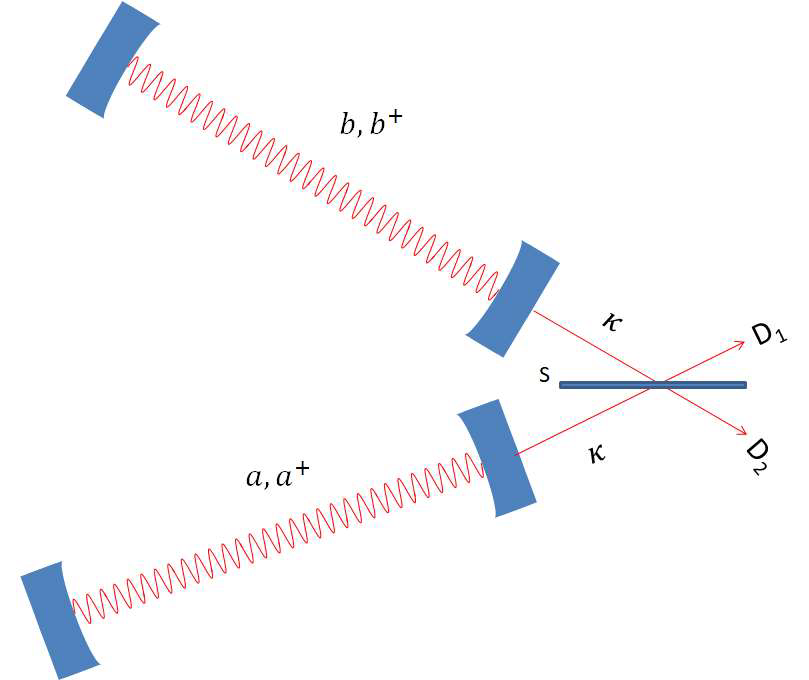
\includegraphics[width=0.5\textwidth]{fig2.png}
    \caption{Output of two cavities are mixed by splitter $S$ and detected by photon-counter $D_1$ and $D_2$}
    \label{fig:prob-2}
\end{figure}

\paragraph{Stochastic wavefunction of two cavity fields} We consider the setup in \prettyref{fig:prob-2}, the leak fields of two identical cavities are mixed by a beamsplitter $S$ and then detected by the photon counter D1 and D2. Following the stochastic wavefunction method, the effective Hamiltonian for the photon field of the twocavity system can be written as $H_{\text {eff }}=\hbar\left(-i \frac{\kappa}{2}\right)\left(a^{+} a+b^{+} b\right)$. While normally we would have quantum jump operators of $C_{a}=\sqrt{\kappa} a$ and $C_{b}=\sqrt{\kappa} b$, here it is more convenient to introduce collective jump operators $C_{1}=\sqrt{\kappa}(t a+r b)$ and $C_{2}=\sqrt{\kappa}\left(-r^{*} a+t b\right)$, with $r, t$ to be the reflective and transmission coefficients of the beamsplitter $S$.

\begin{itemize}
    \item[2.1] Consider the initial state to be a product coherent state: $|\psi(0)\rangle=|\alpha, \beta\rangle$.
    Evaluate the stochastic wavefunction of the photon field, $\left|\psi_{\mathrm{S}}(\mathrm{t})\right\rangle$, for the non-Hermitian evolution without any quantum jump, and after a quantum jump by $C_{1}$ operator (D1 "click")
    \item[2.2] Consider the simple situation of a $50 \%$ beamspitter, $r=t=1 / \sqrt{2}$, continue with the first problem to derive the photon detection rate $\gamma_{1}(t)=\left\langle\psi(t)\left|C_{1}^{+} C_{1}\right| \psi(t)\right\rangle$ and $\gamma_{2}(t)=\left\langle\psi(t)\left|C_{2}^{+} C_{2}\right| \psi(t)\right\rangle$. Is it possible to properly choose non-zero $\alpha$ and $\beta$ values, so as to have $\gamma_{1} \equiv 0$ ?
    \item[2.3] Repeat $2.1$ with the Fock initial state $|\psi(0)\rangle=|N, N\rangle$.
    \item[2.4] Continue with 2.2, again assuming $r=t=1 / \sqrt{2}$, evaluate $\gamma_{1}(t)=\left\langle\psi(t)\left|C_{1}^{+} C_{1}\right| \psi(t)\right\rangle$ and $\gamma_{2}(t)=\left\langle\psi(t)\left|C_{2}^{+} C_{2}\right| \psi(t)\right\rangle$ before there is any quantum jump, and after a quantum jump with a $D_{1}$ "click". For $N=1$. Discuss your results in terms of the HongOu-Mandel effect.
\end{itemize}

\paragraph{Solution} \begin{itemize}
\item[2.1] Following the same procedure in the last problem, we have 
\[
    \ee^{- \kappa (n_a + n_b) t / 2} \ket*{\alpha, \beta} = \ee^{\abs*{\alpha}^2 (\ee^{-\kappa t} - 1) / 2} \ee^{\abs*{\beta}^2 (\ee^{-\kappa t} - 1) / 2} \ket*{\alpha \ee^{- \kappa t / 2}, \beta \ee^{- \kappa t / 2}}, 
\] 
and after normalization we get 
\begin{equation}
    \ket*{\psi(t)}_\text{no jump} = \ket*{\alpha \ee^{- \kappa t / 2}, \beta \ee^{- \kappa t / 2}}.
\end{equation}
After a click, since a coherent state is a eigenstate of the annihilation operator, noting happens and we have 
\begin{equation}
    \ket*{\psi(t)}_\text{jump} = \ket*{\alpha \ee^{- \kappa t / 2}, \beta \ee^{- \kappa t / 2}}.
\end{equation}
\item[2.2] We have 
\[
    \begin{aligned}
        C_1 \ket*{\psi(t)}_\text{no jump} &= \sqrt{\frac{\kappa}{2}} (a + b) \ket*{\alpha \ee^{- \kappa t / 2}, \beta \ee^{- \kappa t / 2}} \\
        &= \sqrt{\frac{\kappa}{2}} (\alpha \ee^{- \kappa t / 2} + \beta \ee^{- \kappa t / 2}) \ket*{\alpha \ee^{- \kappa t / 2}, \beta \ee^{- \kappa t / 2}},
    \end{aligned}
\] 
and therefore before a click, we have 
\begin{equation}
    \gamma_1 = \expval*{C_1^\dagger C_1}{\psi(t)} = \frac{\kappa}{2} \ee^{- \kappa t} \abs*{\alpha + \beta}^2.
\end{equation}
Similarly, 
\[
    \begin{aligned}
        C_2 \ket*{\psi(t)}_\text{no jump} &= \sqrt{\frac{\kappa}{2}} (- a + b) \ket*{\alpha \ee^{- \kappa t / 2}, \beta \ee^{- \kappa t / 2}} \\
        &= \sqrt{\frac{\kappa}{2}} (- \alpha \ee^{- \kappa t / 2} + \beta \ee^{- \kappa t / 2}) \ket*{\alpha \ee^{- \kappa t / 2}, \beta \ee^{- \kappa t / 2}},
    \end{aligned}
\]
and therefore 
\begin{equation}
    \gamma_2 = \expval*{C_2^\dagger C_2}{\psi(t)} = \frac{\kappa}{2} \ee^{- \kappa t} \abs*{\alpha - \beta}^2.
\end{equation}
We see it is possible to always keep $\gamma_1 = 0$, as long as $\alpha + \beta = 0$.
\item[2.3] We have 
\[
    \ee^{- \kappa (n_a + n_b) t / 2} \ket*{N, N} = \ee^{- \kappa (N + N) t / 2} \ket*{N, N},
\]
and therefore after normalization we have 
\begin{equation}
    \ket*{\psi(t)}_\text{jump} = \ket*{N, N}.
\end{equation}
After a click, we have 
\[
    \begin{aligned}
        C_1 \ket*{\psi(t)}_\text{no jump} &= \sqrt{\frac{\kappa}{2}} (t a + r b) \ket*{N, N} \\
        &= \sqrt{\frac{\kappa}{2}} (t \sqrt{N} \ket*{N-1, N} + r \sqrt{N} \ket*{N, N-1}),
    \end{aligned}
\]
and since $\abs*{t}^2 + \abs*{r}^2 = 1$, we have 
\begin{equation}
    \ket*{\psi(t)}_\text{jump} = t \ket*{N-1, N} + r \ket*{N, N-1}.
    \label{eq:n-n-after-jump}
\end{equation}
\item[2.4] We can evaluate $\gamma_1$ and $\gamma_2$ as 
\[
    \begin{aligned}
        \gamma_1 &= \expval*{C_1^\dagger C_1}{\psi(t)} \\
        &= \frac{\kappa}{2} \expval*{(a^\dagger + b^\dagger) (a + b)}{N, N} \\
        &= \frac{\kappa}{2} \times 2 N = \kappa N,
    \end{aligned}
\]  
and 
\[
    \begin{aligned}
        \gamma_2 &= \expval*{C_2^\dagger C_2}{\psi(t)} \\
        &= \frac{\kappa}{2} \expval*{(- a^\dagger + b^\dagger) (- a + b)}{N, N} \\
        &= \frac{\kappa}{2} \times 2 N = \kappa N,
    \end{aligned}
\]  
so 
\begin{equation}
    \gamma_1 = \gamma_2 = \kappa N.
\end{equation}
After a quantum jump, by \eqref{eq:n-n-after-jump}, we have 
\begin{equation}
    \ket*{\psi(t)}_\text{jump} = \frac{1}{\sqrt{2}} (\ket*{N-1,N} + \ket*{N,N-1}).
\end{equation}
We find a measurement entangles two cavities together, and after the jump, we have 
\[
    \begin{aligned}
        \gamma_1 &= \expval{C_1^\dagger C_1}{\psi(t)} \\
        &= \frac{\kappa}{2}  \expval{(a^\dagger + b^\dagger) (a + b)}{\psi(t)}  \\
        &= \frac{\kappa}{4} \abs*{(a + b) (\ket*{N-1, N} + \ket*{N, N-1})}^2,
    \end{aligned}
\]
and since 
\[
    \begin{aligned}
        &\quad (a + b) (\ket*{N-1, N} + \ket*{N, N-1}) \\
        &= \sqrt{N-1} \ket*{N-1, N} + 2 \sqrt{N} \ket*{N-1, N-1} + \sqrt{N-1} \ket*{N, N-2},
    \end{aligned}
\]
we have 
\begin{equation}
    \gamma_1 = \frac{\kappa}{4} \times (N-1 + 4 N + N-1) = \frac{\kappa}{2} (3N-1).
\end{equation}
Similarly, we have 
\[
    \begin{aligned}
        \gamma_2 &= \expval{C_2^\dagger C_2}{\psi(t)} \\
        &= \frac{\kappa}{2}  \expval{(- a^\dagger + b^\dagger) (- a + b)}{\psi(t)}  \\
        &= \frac{\kappa}{4} \abs*{(- a + b) (\ket*{N-1, N} + \ket*{N, N-1})}^2,
    \end{aligned}
\]
and since 
\[
    \begin{aligned}
        &\quad (- a + b) (\ket*{N-1, N} + \ket*{N, N-1}) \\
        &= - \sqrt{N-1} \ket*{N-1, N} + \sqrt{N-1} \ket*{N, N-2},
    \end{aligned}
\]
we have 
\begin{equation}
    \gamma_2 = \frac{\kappa}{4} \times (N-1 + N - 1) = \frac{\kappa}{2} (N-1).
\end{equation}
Note that we do not need to single out the case of $N=1$: terms like $\ket*{N-2}$ automatically vanish because 
of the $\sqrt{N-1}$ factor. When $N=1$, we have 
\begin{equation}
    \ket*{\psi(t)}_\text{jump} = \frac{1}{\sqrt{2}} (\ket*{0, 1} + \ket*{1, 0}),
\end{equation}
and after a $D_1$ click, 
\begin{equation}
    \gamma_1 = \kappa, \quad \gamma_2 = 0.
\end{equation}
This means if we wait and detect another photon, it can only occur at $D_1$. This is an example of observation
induced localization and can be viewed as the asynchronous version of Hong-Ou-Mandel effect. 
\end{itemize}

\paragraph{Discussion} Actually, experimentally all Hong-Ou-Mandel effects can be thought as asynchronous,
as what we really have are partially localized wave packets, and detections of two photons usually happen
at different time points.

\paragraph{}

\begin{figure}
    \centering
    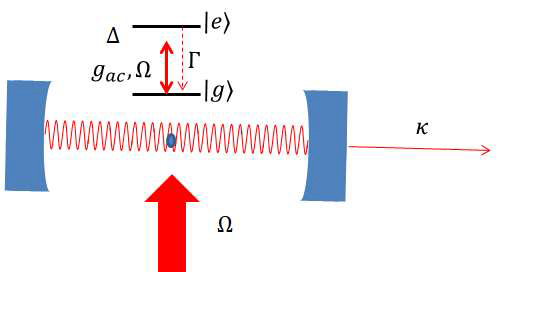
\includegraphics[width=0.7\textwidth]{fig3.png}
    \caption{The device in the third problem}
\end{figure}

\paragraph{Cavity QED and single photon source} As in the figure above, consider a 2-level atom coupled to a cavity field with single-photon Rabi frequency $g_{a c}$. The atom is in addition subjected to a laser field excitation from the side with a Rabi frequency $\Omega(\mathrm{t})$. Taking into account the radiative decay by the atom and the leak of the cavity, the effective Hamiltonian of the controlled and coupled system is given by
\begin{equation}
    H_\text{eff}=\hbar\left(- \ii \frac{\Gamma}{2}\right)|e\rangle\langle e|+\hbar\left(-\Delta- \ii \frac{\kappa}{2}\right) a^{+} a+\left[\hbar\left(\frac{\Omega(\mathrm{t})}{2}+g_{a c} a\right)|e\rangle\langle g|+\text { h.c. }\right],
\end{equation}
where $\Delta=\omega-\omega_{e g}$ is the detuning of the cavity mode frequency from the atomic resonant frequency. The collapse operators are given by $C_{1}=\sqrt{\Gamma}|g\rangle\langle e|$ and $C_{2}=\sqrt{\kappa} a$.
3a) Consider $\Omega(\mathrm{t})=0$ and with system initially in $\left|\psi_{S}(0)\right\rangle=|g, n=1\rangle$, that is, the atom is in the ground state and the cavity mode is in $\mathrm{n}=1$ Fock state. Consider good cavity $(\kappa \ll g, \Gamma)$ and weak coupling $(g \ll \Delta, \Gamma)$ limits. Expand $\left|\psi_{S}(t)\right\rangle$ in proper basis of choice, and to derive the Schrodinger equation for the coefficients of the stochastic wavefunction, without quantum jump. Perturbatively derive the system decay rate $ \gamma_{1}(t)=\left\langle\psi_{S}\left|C_{1}^{+} C_{1}\right| \psi_{S}\right\rangle$ and $ \gamma_{2}(t)=\left\langle\psi_{S}\left|C_{2}^{+} C_{2}\right| \psi_{S}\right\rangle$ (i.e., using the adiabatic elimination method which assumes $\left|\psi_{S}(t)\right\rangle \approx\left|\widetilde{\psi}_{S}\right\rangle$, with $\left.H_\text{eff}\left|\widetilde{\psi_{S}}\right\rangle \approx-\Delta-\frac{i \kappa}{2}\left|\widetilde{\psi_{S}}\right\rangle\right)$.
3b) Repeat Question 3a, but with system initially in $|\psi\rangle=|e, n=0\rangle$ and in the bad cavity $(\kappa >> g, \Gamma)$ and weak coupling $(g \ll \Delta, \Gamma)$ limit. You should arrive at a total decay rate $\gamma=\gamma_{1}+\gamma_{2}$ that describes the Purcell effect as in the class. Discuss the condition under which $\gamma_{2} \gg \gamma_{1}$, that is, the decay of the system more likely leading to a single photon emission into the cavity leak mode.
3c) With the system initially in $|\psi\rangle=|g, n=0\rangle$ and with a resonant pulse $\Omega(t)=$ $\Omega_{0} \sin \left(\frac{\pi t}{\tau}\right)$ switched on and off smoothly for $0<t<\tau$. Assuming $|\psi(t)\rangle$ to be driven by the 2-level Hamiltonian $H_{a}=H_{e f f}(t ; \Gamma, \kappa, g \rightarrow 0) \quad$ [note: this happens effectively when $\Gamma, \kappa, g \ll$ $1 / \tau]$. Now, putting back all the parameters into $H_\text{eff}$, Calculate $\gamma_{1}(t)=\left\langle\psi\left|C_{1}^{\dagger} C_{1}\right| \psi\right\rangle$ and $\gamma_{2}(t)=\left\langle\psi\left|C_{2}^{\dagger} C_{2}\right| \psi\right\rangle$ for stochastic wavefunction without quantum jump during $0<\mathrm{t}<\mathrm{T}$, with $T \gg \frac{1}{\kappa}, \frac{1}{\Gamma}$
4d) Discuss $\Omega(t)$ and other parameters in Eq. (2), so that a single photon can be deterministically generated into the cavity leaking mode with high efficiency. Discuss the form of the single-photon wavefunction, and the fidelity of the single-photon source (how likely there is exactly one photon in the time-dependent leaky mode).

\paragraph{Solution} \begin{itemize}
\item[(a)] It is easy to find that only $\ket*{e, n=0}$ and $\ket*{g, n=1}$ have coupling. With the basis 
$\{ \ket*{g, n=1}$, $\ket*{e, n=0} \}$, we have 
\begin{equation}
    H_\text{eff} = \pmqty{ - \hbar (\Delta + \ii \kappa / 2) & \hbar g_{ac}^* \\ \hbar g_{ac} & - \ii \hbar \Gamma / 2 }.
    \label{eq:heff-subspace-1}
\end{equation} 
The correction of the energy of $\ket*{e, n=0}$ is of $\bigO(g_{ac}^2 / \Gamma)$ order, and we can just throw 
it away. On the other hand, the coupling between $\ket*{g, n=1}$ and $\ket*{e, n=0}$ has a first order correction
to $\ket*{g, n=1}$, which possibly contributes a non-zero term to $\gamma_1$. So what we need to do is to find 
the eigenstate correction. 

Suppose 
\[
    \ket*{\psi_\text{S}(t)} = c_g \ket*{g, n=1} + c_e \ket*{e, n=0}.
\]
Since there is no energy correction, we have 
\[
    \ii \dot{c}_g = (- \Delta - \ii \kappa / 2) c_g, \quad \ii \dot{c}_e = (- \Delta - \ii \kappa / 2) c_e.
\]
On the other hand, \eqref{eq:heff-subspace-1} gives 
\[
    \ii \hbar \dot{c}_e = \hbar g_{ac} c_g - \ii \hbar \Gamma / 2 \times c_e,
\]
and therefore we have 
\[
    \frac{\ii \Gamma - 2 \Delta - \ii \kappa}{2 } c_e = g_{ac} c_g \approx g_{ac},
\]
where we have omitted the time evolution factor of $c_g$, which is fine since both $c_e$ and $c_g$ evolve in 
the same pace, and the normalization after each time step can wipe away factors like $\ee^{- \Gamma t / 2}$,
and we have 
\[
    c_e = \frac{2 g_{ac}}{\ii \Gamma - 2 \Delta - \ii \kappa},
\]
\begin{equation}
    \ket*{\psi(t)} \approx \ket*{g, n=1} + \frac{2 g_{ac}}{\ii \Gamma - 2 \Delta - \ii \kappa} \ket*{e, n=0}.
\end{equation}
This is a (quasi)stationary state, and no further normalization is required, since there is no quantum jump 
and therefore no total probability loss. We have 
\[
    \begin{aligned}
        \gamma_1 &= \Gamma \braket*{\psi}{e} \braket*{e}{\psi} = \Gamma \abs*{c_e}^2 \\
        &= \Gamma \abs{\frac{2 g_{ac}}{\ii \Gamma - 2 \Delta - \ii \kappa}}^2 \\
        &= \Gamma \frac{4 \abs*{g_{ac}}^2}{(\Gamma - \kappa)^2 + 4 \Delta^2 },
    \end{aligned}
\]
so
\begin{equation}
    \gamma_1 = \Gamma \frac{4 \abs*{g_{ac}}^2}{(\Gamma - \kappa)^2 + 4 \Delta^2 } \approx \Gamma \frac{4 \abs*{g_{ac}}^2}{\Gamma^2 + 4 \Delta^2 }.
    \label{eq:gamma-1-1}
\end{equation}
Also, 
\begin{equation}
    \gamma_2 = \kappa \expval{a^\dagger a}{\psi} = \kappa.
\end{equation}
So we can see the leading order contribution of the coupling between $\ket*{g, n=1}$ and $\ket*{e, n=0}$ is 
\eqref{eq:gamma-1-1}.

\begin{note*}{}
    Note that the so-called adiabatic elimination gives a $\bigO(g_{ac})$ correction to the eigenstates,
    and this can be obtained equivalently by an ordinary perturbative calculation. We call it \emph{adiabatic}
    because what we are doing is actually assuming $c_e$ evolves synchronously with $c_g$, or in other words
    $c_{g}$ adiabatically ``drags'' $c_{e}$. 
    It can be proved that adiabatic elimination, time independent perturbation theory, and path integral 
    all give the same results.
\end{note*}

\item[(b)] Now we repeat the argument in (a) and make no energetic correction to $\ket*{e, n=0}$. Suppose 
$\ket*{\psi(t)} = c_e \ket*{e, n=0} + c_g \ket*{g, n=1}$, and the approximate time evolution equations are 
\[
    \ii \hbar \dot{c}_e = - \ii \hbar \Gamma / 2 c_e, \quad \ii \hbar \dot{c}_g = - \ii \hbar \Gamma / 2 c_g.
\]
On the other hand we have the exact evolution equation of $c_g$, which is 
\[
    \ii \hbar \cdot{c}_g = - \hbar (\Delta + \ii \kappa / 2) c_g + \hbar g_{ac}^* c_a,
\]
and we have 
\[
    c_g = \frac{g_{ac}^*}{\Delta + \ii \kappa / 2 - \ii \Gamma / 2} c_e \approx \frac{g_{ac}^*}{\Delta + \ii \kappa / 2 - \ii \Gamma / 2}.
\]
Therefore we have 
\begin{equation}
    \ket*{\psi(t)} = \ket*{e, n=0} + \frac{g_{ac}^*}{\Delta + \ii \kappa / 2 - \ii \Gamma / 2} \ket*{g, n=1},
\end{equation}
again a quasi-stationary state. The scattering rates are 
\begin{equation}
    \gamma_1 = \Gamma \abs*{\braket*{\psi}{e}}^2 \approx \Gamma ,
\end{equation}
and 
\begin{equation}
    \gamma_2 = \kappa \expval*{a^\dagger a}{\psi(t)} = \kappa \abs*{c_g}^2 = \kappa \frac{4 \abs*{g_{ac}}^2}{4 \Delta^2 + (\kappa - \Gamma)^2} \approx \kappa \frac{4 \abs*{g_{ac}}^2}{4 \Delta^2 + \kappa^2} .
\end{equation}
Therefore we find 
\begin{equation}
    \gamma = \Gamma + \kappa \frac{4 \abs*{g_{ac}}^2}{4 \Delta^2 + \kappa^2}.
\end{equation}
We see that the existence of the cavity gives rise to the $a$ and $a^\dagger$ modes, which in turn give rise 
to the $a \dyad*{e}{g}$ term in the Hamiltonian, which dresses the excited state, and it is exactly the 
correction term $c_g \ket*{g, n=1}$ in $\ket*{\psi(t)}$ (which is the dressed excited state) that contributes 
a non-zero value to $\gamma_2$. Therefore, we see the cavity increases the probability of quantum jump, which 
is an instance of Purcell effect.

\item[(c)] We can divide the time span $0 < t < T$ into $0 < t < \tau$ and $\tau < t < T$.
 
During the $0 < t < \tau$ period, $\Omega(t)$ is almost the main interacting channel, and since $\tau$ is small,
we may assume there is no photon emission into the cavity or quantum jump during this period.
Therefore, there is no coupling between states with different photon numbers, and we can just throw away 
the $a^\dagger a$ term, and work in the subspace spanned by $\{\ket*{g, n=0}, \ket*{e, n=0}\}$, in which 
the Hamiltonian is 
\begin{equation}
    H_\text{eff} = \frac{\hbar}{2} \pmqty{ 0 & \Omega^*(t) \\ \Omega(t) & 0 } 
    = \frac{\hbar}{2} \Omega_0 \sin(\frac{\pi t}{\tau}) \sigma^x .
\end{equation} 
The time evolution operator of components of the wave function is 
\[
    \begin{aligned}
        \exp(- \frac{\ii}{\hbar} \int_0^t \dd{t'} H_\text{eff}(t')) &= 
        \exp(- \frac{\ii \Omega_0}{2} \sigma^x \int_0^t \dd{t'} \sin(\frac{\pi t'}{\tau}) ) \\
        &= \exp(- \frac{\ii \Omega_0}{2} \sigma^x \frac{\tau}{\pi} \left( 1 - \cos(\frac{\pi t}{\tau}) \right)) \\
        &= \cos(\frac{\Omega_0}{2} \frac{\tau}{\pi} \left( 1 - \cos(\frac{\pi t}{\tau}) \right))
        - \ii \sigma_x \sin(\frac{\Omega_0}{2} \frac{\tau}{\pi} \left( 1 - \cos(\frac{\pi t}{\tau}) \right)),
    \end{aligned}
\]
and applying this operator to $\ket*{\psi(0)} = (1, 0)$, we get 
\begin{equation}
    \ket*{\psi(t)} = \cos \theta(t) \ket*{g, n=0} - \ii \sin \theta(t) \ket*{e, n=0}, 
\end{equation}
where 
\begin{equation}
    \theta(t) = \frac{\Omega_0}{2} \frac{\tau}{\pi} \left( 1 - \cos(\frac{\pi t}{\tau}) \right).
\end{equation}
The scattering rates are 
\begin{equation}
    \gamma_1 = \Gamma \abs*{\braket*{\psi}{e}}^2 = \Gamma \sin^2 \theta(t),
\end{equation}
and 
\begin{equation}
    \gamma_2 = \kappa \expval*{n_a}{\psi} = 0.
\end{equation}

When $t = \tau$, we have 
\begin{equation}
    \ket*{\psi(\tau)} = \cos \frac{\Omega_0 \tau}{\pi} \ket*{g, n=0} - \ii \sin \frac{\Omega_0 \tau}{\pi} \ket*{e, n=0}.
    \label{eq:tau-init}
\end{equation}
This is the initial value of the time evolution from $\tau$ to $t$, where $\Omega(t)$ is turned down and the 
Hamiltonian is 
\begin{equation}
    H_\text{eff} = - \ii \hbar \frac{\Gamma}{2} \dyad{e} + \hbar \left(- \Delta - \frac{\ii \kappa}{2}\right) a^\dagger a + \hbar g_{ac} a \dyad{e}{g} + \text{h.c.}.
\end{equation}
We can see that from $\ket*{g, n=0}$ and $\ket*{e, n=0}$, by a $a^\dagger \dyad*{g}{e}$ process we can reach 
$\ket*{g, n=1}$. On the other hand, $\ket*{g, n=0}$ is isolated: it cannot be turned into any other state and
without quantum jumps, no state can jump to it. We have $H_\text{eff} \ket*{g, n=0} = 0$, and the $\ket*{g, n=0}$
component in \eqref{eq:tau-init} evolves trivially. The effective Hamiltonian on the subspace spanned by 
$\{\ket*{g, n=1}, \ket*{e, n=0}\}$ is 
\begin{equation}
    \begin{aligned}
        H_\text{eff} &= \pmqty{ - \hbar (\Delta + \ii \kappa / 2) & \hbar g_{ac}^* \\ \hbar g_{ac} & - \ii \hbar \Gamma / 2 } \\
        &= - \frac{1}{2} \hbar \left( \Delta + \frac{\ii \hbar (\kappa + \Gamma)}{2} \right) \sigma^0 + 
        \hbar \Re g_{ac} \sigma^x + \hbar \Im g_{ac} \sigma^y + \frac{1}{2} \underbrace{\left( - \hbar \Delta + \frac{\ii \hbar (\Gamma - \kappa)}{2} \right)}_{\eqqcolon \hbar \tilde{\Delta}} \sigma^z.
    \end{aligned}
\end{equation}
We define (the reason can be found in \href{../4/4.pdf}{the last homework})
\begin{equation}
    \vb*{\Omega} = (2 \Re g_{ac}, 2 \Im g_{ac}, \tilde{\Delta}), \quad \tilde{\Omega} = \sqrt{\tilde{\Delta}^2 + 4 \abs*{g_{ac}}^2} , \quad \vb*{n} = \frac{\vb*{\Omega}}{\tilde{\Omega}},
\end{equation}
and we have 
\[
    \begin{aligned}
        \exp(- \ii \frac{t - \tau}{\hbar} H_\text{eff}) &= \exp(\frac{t - \tau}{2} \left( \ii \Delta - \frac{\Gamma + \kappa}{2} \right)) \exp(- \frac{\ii (t - \tau) \vb*{\Omega} \cdot \vb*{\sigma}}{2}) \\
        &= \exp(\frac{t - \tau}{2} \left( \ii \Delta - \frac{\Gamma + \kappa}{2} \right)) \left( \cos(\frac{(t - \tau) \tilde{\Omega}}{2}) - \ii \vb*{n} \cdot \vb*{\sigma} \sin(\frac{(t - \tau) \tilde{\Omega}}{2}) \right),
    \end{aligned}
\]
and since 
\[
    \vb*{n} \cdot \vb*{\sigma} \ket*{e, n=0} = (n_x - \ii n_y) \ket*{g, n=1} - n_z \ket*{e, n=0},
\]
we have 
\[
    \begin{aligned}
        &\exp(- \ii \frac{t - \tau}{\hbar} H_\text{eff}) \ket*{e, n=0} = \exp(\frac{t - \tau}{2} \left( \ii \Delta - \frac{\Gamma + \kappa}{2} \right)) \\
        &\quad \quad \times \left( \left( \cos \frac{(t - \tau) \tilde{\Omega}}{2} - \ii \sin \frac{(t - \tau) \tilde{\Omega}}{2} n_z \right) \ket*{e, n=0} - \ii \sin \frac{(t - \tau) \tilde{\Omega}}{2} (n_x - \ii n_y) \ket*{g, n=1} \right). 
    \end{aligned}
\]
So 
\begin{equation}
    \ket*{\psi(t)} = \frac{C_1 \ket*{g, n=0} + C_2 \ket*{g, n=1} + C_3 \ket*{e, n=0}}{\sqrt{\abs*{C_1}^2 + \abs*{C_2}^2 + \abs*{C_3}^2}} , 
\end{equation}
where 
\begin{equation}
    C_1 =  \cos \frac{\Omega_0 \tau}{\pi} \ket*{g, n=0},
\end{equation}
\begin{equation}
    C_2 = -  \sin \frac{\Omega_0 \tau}{\pi} \ket*{g, n=0} \exp(\frac{t - \tau}{2} \left( \ii \Delta - \frac{\Gamma + \kappa}{2} \right)) \sin \frac{(t - \tau) \tilde{\Omega}}{2} (n_x - \ii n_y) ,
    \label{eq:c2}
\end{equation}
and 
\begin{equation}
    C_3 = - \ii \sin \frac{\Omega_0 \tau}{\pi} \exp(\frac{t - \tau}{2} \left( \ii \Delta - \frac{\Gamma + \kappa}{2} \right)) \left( \cos \frac{(t - \tau) \tilde{\Omega}}{2} - \ii \sin \frac{(t - \tau) \tilde{\Omega}}{2} n_z \right) .
    \label{eq:c3}
\end{equation}
We have 
\begin{equation}
    \gamma_1 = \Gamma \frac{\abs*{C_3}^2}{\abs*{C_1}^2 + \abs*{C_2}^2 + \abs*{C_3}^2},
\end{equation}
and 
\begin{equation}
    \gamma_2 = \kappa \frac{\abs*{C_2}^2}{\abs*{C_1}^2 + \abs*{C_2}^2 + \abs*{C_3}^2}.
\end{equation}

\item[(d)] We want to maximize the probability to find a photon in the cavity, so that it can leak out.
To achieve this, we need to make $C_1$ and $C_3$ as small as possible, which can be done by choosing 
\begin{equation}
    \frac{\Omega_0 \tau}{\pi} = \frac{\pi}{2}.
\end{equation}
In this case, we can throw away common factors in \eqref{eq:c2} and \eqref{eq:c3}, and now the wave function 
is 
\begin{equation}
    \ket*{\psi(t)} = \frac{1}{C} \sin \frac{(t - \tau) \tilde{\Omega}}{2} (n_x - \ii n_y) \ket*{g, n=1} + \frac{\ii}{C} \left( \cos \frac{(t - \tau) \tilde{\Omega}}{2} - \ii \sin \frac{(t - \tau) \tilde{\Omega}}{2} n_z \right) \ket*{e, n=0},
\end{equation}
where $C$ is a normalization constant. 

\end{itemize}

\paragraph{Discussion} Actually we can find the single photon wave function of the leaked photon, which is like 
\begin{equation}
    \vb*{E} \propto \theta\left(t - \frac{r}{c}\right) \ee^{- \kappa(t - r / c) / 2}.
\end{equation}

\end{document}